\chapter{System Architecture and Design}
{\itshape Achieving real-time video segmentation requires a design that decouples computational execution from user interaction. A high-level overview of the architectural decisions behind this framework is presented, detailing how a modular pipeline separates the classical and quantum-inspired clustering engines. This decoupled backend integrates with an interactive, immediate-mode user interface, enabling real-time parameter tuning and direct performance comparisons without introducing latency in the rendering loop.}

\section{Architectural Overview}
The segmentation framework is designed as a high-throughput, asynchronous pipeline that processes live camera feeds with minimal latency. To keep the user interface responsive during heavy GPU calculations, the application decouples the GUI from the computational backend. This separation is implemented using a multi-threaded architecture with a dedicated worker thread, as shown in Figure~\ref{fig:system_architecture}.

\begin{figure}[htbp]
\centering
\resizebox{\textwidth}{!}{%
\begin{tikzpicture}[
    node distance = 1.0cm and 0.8cm,
    auto,
    % Box Styles
    layerBox/.style = {rectangle, draw, rounded corners=4, line width=1.2pt, inner sep=0.5cm},
    nodeBox/.style = {rectangle, draw, rounded corners=2, minimum height=0.8cm, fill=white, text width=3.2cm, align=center, font=\small},
    subBox/.style = {rectangle, draw, dashed, rounded corners=2, minimum height=1.4cm, text width=4.5cm, align=center, font=\small},
    % Arrow Style
    dataLine/.style = {-{Stealth[scale=1.2]}, line width=1pt, draw=black!80}
]

    % ==========================================
    % LAYER 1: WORKER & CUDA PIPELINE (TOP PANEL)
    % ==========================================
    \node[nodeBox, fill=purple!10, draw=purple!80] (CV) {Worker Thread Loop \\ (OpenCV Capture)};
    \node[nodeBox, fill=purple!10, draw=purple!80, right=of CV] (Prep) {Preprocessor Staging \\ (Strided Prep)};
    \node[subBox, fill=cyan!8, draw=cyan!60!black, right=of Prep] (DMA) {Asynchronous DMA \\ \scriptsize cudaMemcpyAsync over stream};
    \node[subBox, fill=green!5, draw=green!50, right=of DMA] (GPU) {GPU Device Kernels \\ \scriptsize K-Means Engines};

    \path[dataLine] (CV) -- (Prep);
    \path[dataLine] (Prep) -- (DMA);
    \path[dataLine] (DMA) -- (GPU);

    % ==========================================
    % LAYER 2: SYNCHRONIZATION BRIDGE (MIDDLE PANEL)
    % ==========================================
    \node[nodeBox, fill=orange!10, draw=orange!80, below=3.0cm of CV] (CfgL) {std::scoped\_lock \\ (m\_configMutex)};
    \node[nodeBox, fill=orange!10, draw=orange!80, below=3.0cm of GPU] (DataL) {std::scoped\_lock \\ (m\_dataMutex)};

    % ==========================================
    % LAYER 3: UI THREAD (BOTTOM PANEL)
    % ==========================================
    \node[nodeBox, fill=blue!10, draw=blue!80, below=3.0cm of CfgL] (GLFW) {GLFW Context \\ (Event Loop)};
    \node[nodeBox, fill=blue!10, draw=blue!80, below=3.0cm of DataL] (Views) {GUI Dashboards \\ (Panels \& Overlays)};
    \path (GLFW.center) -- (Views.center) coordinate[midway] (MidUI);
    \node[nodeBox, fill=blue!10, draw=blue!80] (ImGui) at (MidUI) {Dear ImGui \\ (Immediate Mode)};

    \path[dataLine] (GLFW) -- (ImGui);
    \path[dataLine] (ImGui) -- (Views);

    % Coordinates for container top clearance
    \path (CV.north) ++(0,0.8) coordinate (L1Top);
    \path (CfgL.north) ++(0,0.8) coordinate (L2Top);
    \path (GLFW.north) ++(0,0.8) coordinate (L3Top);

    % ==========================================
    % BACKGROUND CONTAINERS
    % ==========================================
    \begin{pgfonlayer}{background}
        % Layer 2 first so L1 can reference its extents
        \node[layerBox, fill=orange!5, draw=orange!60,
              fit=(CfgL) (DataL) (L2Top)
                  (GPU.south east |- DataL) (CV.south west |- CfgL)] (L2) {};

        % Layer 1 — forced to match L2's horizontal extents
        \node[layerBox, fill=purple!5, draw=purple!60,
              fit=(CV) (GPU) (L1Top)
                  (L2.north west |- CV) (L2.north east |- GPU)] (L1) {};

        % Layer 3 — forced to match L2's horizontal extents
        \node[layerBox, fill=blue!5, draw=blue!60,
              fit=(GLFW) (Views) (ImGui) (L3Top)
                  (L2.south west |- GLFW) (L2.south east |- Views)] (L3) {};
    \end{pgfonlayer}

    % Layer titles
    \node[purple!80, font=\bfseries\small, anchor=north west, xshift=0.3cm, yshift=-0.2cm] at (L1.north west) {Worker \& CUDA Pipeline Core};
    \node[orange!80, font=\bfseries\small, anchor=north west, xshift=0.3cm, yshift=-0.2cm] at (L2.north west) {Thread Synchronization Bridge};
    \node[blue!80, font=\bfseries\small, anchor=north west, xshift=0.225cm, yshift=-0.2cm] at (L3.north west) {UI Thread (Main Render Loop)};

    % ==========================================
    % INTER-LAYER ROUTING LINES
    % ==========================================
    \draw[dataLine, color=orange!80!black] (GLFW.north) -- (CfgL.south)
        node[text width=2.8cm, pos=0.6, left, xshift=3.2cm, font=\scriptsize\sf] {1. Mutates Parameters (optional)};
    \draw[dataLine, color=purple!80] (CfgL.north) -- (CV.south)
        node[text width=2.8cm, pos=0.6, left, xshift=3.2cm, font=\scriptsize\sf] {2. Updates Hyperparameters (optional)};
    \draw[dataLine, color=orange!80!black] (GPU.south) -- (DataL.north)
        node[text width=3.5cm, pos=0.5, right, font=\scriptsize\sf] {3. Commits Staged VRAM Data};
    \draw[dataLine, color=blue!70!black] (DataL.south) -- (GLFW.north)
        node[sloped, above, pos=0.5, font=\scriptsize\sf] {4. Pulls Textures};

\end{tikzpicture}%
}
\caption{Dual-Threaded Architecture with Asynchronous CUDA Pipeline Staging}
\label{fig:system_architecture}
\end{figure}

\subsection{Technological Stack}
The framework is built using C++20 and the NVIDIA CUDA toolkit \cite{CudaGuide} to handle the intense processing demands of 5D pixel clustering. C++20 features like \texttt{std::span} are used to pass memory-safe views of host-resident buffers without the overhead of deep copies \cite{stroustrup2022tour}. This high-performance stack allows the system to process hundreds of thousands of pixels in parallel, bypassing the traditional single-threaded CPU bottlenecks.

\subsection{Thread Partitioning and Asynchronous Pipeline}
To achieve real-time performance, the application runs on two main threads that communicate asynchronously:
\begin{itemize}
    \item \textbf{UI Thread (Main):} Handles the application lifecycle, processes window events, and renders the immediate-mode GUI using Dear ImGui \cite{ImGui}. It retrieves fully processed segmented frames from shared buffers using a mutex-protected synchronization lock \cite{williams2019c++}.
    \item \textbf{Clustering Worker Thread:} Managed by the core \texttt{Application} class, this thread runs the main clustering loop. It continuously updates hyperparameters from the UI, executes the active CUDA clustering engine, and commits the resulting segmented frames to shared buffers for UI rendering.
\end{itemize}

The execution follows a clean four-stage data lifecycle. First, a new frame is captured using OpenCV \cite{Bradski2000} and uploaded to the GPU as a 5D feature set. Second, the \texttt{ClusteringManager} dispatches the active \texttt{KMeansEngine} to run optimized CUDA kernels for pixel assignment. Third, instead of transferring pixel labels back to the CPU, a custom kernel re-colors the pixels directly on the GPU. Finally, the processed frame is transferred back to host memory using page-locked (pinned) memory (allocated via \texttt{cudaMallocHost}) to minimize PCIe transfer overhead, and the UI thread uploads it to an OpenGL texture for real-time rendering \cite{CudaGuide}.

\section{Design Patterns and Core Principles}
Specific software design patterns are used to decouple mathematical engines from the GUI, ensuring the system is modular and easy to maintain \cite{gamma1995design}.

\subsection{Creational and Structural Patterns}
The creation and interchangeability of the components are decoupled using the following structural principles:
\begin{itemize}
    \item \textbf{Factory Method:} The \texttt{ClusteringFactory} encapsulates the instantiation of the computational engines and initialization strategies based on runtime configuration enums \cite{gamma1995design}. This prevents the high-level application from depending directly on concrete CUDA engine classes.
    \item \textbf{Strategy Pattern:} The clustering and initialization algorithms are implemented as interchangeable strategies \cite{gamma1995design}. This allows for swapping the classical Euclidean engine with the quantum-inspired engine at runtime without interrupting the video capture pipeline.
    \item \textbf{Facade Pattern:} The \texttt{ClusteringManager} is a simplified, high-level interface to the complex GPU subsystems (preprocessing, kernel dispatching, and VRAM management) \cite{gamma1995design}.
    \item \textbf{Bridge Pattern (Pimpl):} The Pointer to Implementation (Pimpl) idiom is used in the manager classes as a form of the Bridge Pattern \cite{gamma1995design}. This is a compiler firewall, hiding CUDA-specific types and OpenCV headers from the global project scope, which keeps compile times low \cite{stroustrup2022tour}.
\end{itemize}

\subsection{Behavioral and Concurrency Patterns}
For asynchronous execution and clean resource handling, the system implements:
\begin{itemize}
    \item \textbf{Command Pattern:} Benchmark requests are encapsulated into \texttt{Benchmark\allowbreak Command} objects. This allows for queuing and executing performance comparisons asynchronously without locking the UI \cite{gamma1995design}.
    \item \textbf{Observer Pattern:} The \texttt{BenchmarkRunner} is a subject that broadcasts benchmark results to the GUI as they complete, keeping the benchmarking engine decoupled from the UI widgets \cite{gamma1995design}.
    \item \textbf{Resource Acquisition Is Initialization (RAII):} The \texttt{CudaAssignmentContext} manages the lifetime of all GPU resources. It handles the automatic allocation and deterministic release of device memory (VRAM) and page-locked host memory, preventing memory leaks in high-frequency loops \cite{stroustrup2022tour}.
\end{itemize}

\section{Feature Space and Data Engineering}
The success of clustering depends entirely on how the input data is represented. The framework moves beyond simple RGB grouping by constructing a 5D manifold that balances color and space.

\subsection{The Normalized 5D Manifold}\label{subsect:normalized_manifold}
As derived in Section~\ref{subsect:manifold}, each pixel is mapped to a normalized 5D feature vector $\mathbf{x}_n = [B_n, G_n, R_n, \lambda x_n, \lambda y_n]^T$. The data engineering pipeline, implemented in \texttt{StridedDataPreprocessor}, normalizes color values to $[0, 1]$ by multiplying the raw BGR values by $1/255$. Spatial coordinates are similarly mapped to $[0, 1]$ using the reciprocal of the processing dimensions. 

To prevent geometric coordinates from dominating the distance calculations on high-resolution frames, a spatial scaling weight ($\lambda_{\text{spatial}} = 10^{-6}$) is applied. This weight ensures that chromatic similarity drives the segmentation, while spatial information acts as a regularizer to prevent noisy, fragmented pixel regions \cite{shi2000normalized, achanta2012slic}.

\subsection{Phase Mapping for the Quantum Engine}
For the quantum-inspired backend, the normalized 5D coordinates are mapped to angular phase states: $\theta_d = (p_d - c_d) \cdot \lambda_{\text{scale}}$, where $\lambda_{\text{scale}} = \pi/4$. As detailed in Section~\ref{subsect:phasespace}, this maps the classical feature differences into a bounded angular domain. The GPU engine uses this mapping to calculate non-linear similarity overlaps via hardware-accelerated cosine intrinsics \cite{CudaGuide}, which is designed to help preserve edge transitions under noisy conditions.

\subsection{Strided Sampling for Dimensionality Reduction}
To keep the frame rate stable, the iterative centroid learning phase is decoupled from the final pixel assignment phase. Centroid learning is performed on a subsampled sparse manifold generated by the preprocessor (using the parallel strided downsampling theory detailed in Section~\ref{subsect:downsampling_theory}), while final assignment is run on the full target resolution \cite{achanta2012slic}.

The preprocessor samples the frame at regular spatial strides $S \in [1, 16]$. This reduces the total number of points in the learning feature space by a factor of $S^2$, substantially reducing computational complexity. Statistically, by the Law of Large Numbers, this uniform subsampling of thousands of pixels remains highly representative of the image's overall color-spatial distribution, ensuring that the estimated centroids approximate the true global cluster centers with high fidelity \cite{mouton2020stride}. The resulting sparse manifold is uploaded to the GPU as a contiguous memory block, which enables fast, coalesced memory access \cite{CudaGuide}.

\section{Component Specifications}
The C++/CUDA implementation is organized into modular classes that separate the parallel mathematical solvers from the dashboard user interface.

\subsection{ClusteringManager (The Orchestrator)}
The \texttt{ClusteringManager} coordinates the entire segmentation lifecycle. It implements the Pimpl idiom to isolate raw CUDA device pointers from the rest of the application \cite{stroustrup2022tour, meyers2014effective}. The manager also handles temporal consistency across frames: it caches the converged centroids from the previous video frame to use as the starting seeds for the current frame. This warm-start strategy significantly reduces the number of iterations needed for convergence in live streams.

\subsection{CudaAssignmentContext (The Resource Container)}
The \texttt{CudaAssignmentContext} is the core RAII resource handler \cite{stroustrup2022tour}. It manages GPU memory allocations (VRAM) and page-locked host memory buffers. At runtime, the context dynamically calculates the shared memory requirements for the kernels based on the active cluster count $K$. This keeps the shared centroid cache perfectly sized, maximizing GPU occupancy and minimizing VRAM lookup latency \cite{CudaGuide}.

\subsection{Engine Hierarchy and Factory}
The computational core is structured around an abstract \texttt{KMeansEngine} base class, which defines a strict execution contract for all backend variants:
\begin{itemize}
    \item \textbf{ClassicalEngine:} Implements the parallel Euclidean-based Lloyd iterations. It leverages thread-level parallelism on the GPU to calculate distances for all pixels simultaneously \cite{farivar2008parallel}.
    \item \textbf{QuantumEngine:} Implements the phase-encoded fidelity metric, using single-cycle hardware-accelerated cosine intrinsics \cite{CudaGuide} to evaluate state-overlaps in simulated Hilbert space.
\end{itemize}
These engines are instantiated dynamically by the \texttt{ClusteringFactory}, allowing the user to swap the active algorithm at runtime without interrupting the pipeline.

\subsection{StridedDataPreprocessor}
The \texttt{StridedDataPreprocessor} is the bridge between OpenCV's CPU buffers \cite{Bradski2000} and the GPU's feature arrays. It extracts BGR values, applies spatial scaling, and downsamples the data using the strided sampling strategy.

The preprocessor organizes the features into an AoS format, where the five features ($B, G, R, x, y$) for each pixel are stored contiguously. Although this AoS layout introduces a strided access pattern across the warp (as threads access memory with a stride of five elements), it maximizes $L_1$/$L_2$ cache line utilization for individual threads. Because a single thread requires all five features simultaneously for its distance calculation, fetching the first coordinate pulls the remaining contiguous features into the cache line, minimizing subsequent global VRAM transactions and hiding memory latency \cite{CudaGuide}.

\subsection{User Interface and Telemetry Layer}\label{subsect:ui_telemetry}
The GUI dashboard is implemented using Dear ImGui \cite{ImGui}, providing a lightweight control layer that runs directly inside the GLFW \cite{GLFWdocs} loop. Decoupling is maintained by the \texttt{UIManager} class, which manages three main components:
\begin{itemize}
    \item \textbf{VideoFeedUI:} Renders the real-time segmented GPU textures asynchronously. Representative segmented output frames and visual comparisons are detailed in Section~\ref{subsect:cross_dataset_quality_telemetry} and Case Study I (Section~\ref{subsect:case_study_1}).
    \item \textbf{ControlPanelUI:} Provides widgets to adjust the cluster count ($K$), stride parameter ($S$), and learning interval. It also handles engine switching, provides buttons to toggle centroid overlays and reset centroid coordinates, displays live telemetry (FPS, engine latency, and render times), and provides the control trigger to initiate the side-by-side benchmark comparison. The layout of this control dashboard and its integrated telemetry readouts are displayed in Figure~\ref{fig:control_panel}.
    \item \textbf{BenchmarkOverlayUI:} Renders a full-screen overlay showing the original still frame alongside both segmented engine outputs. It displays comparative telemetry (quality metrics, latencies, and iteration counts) and provides controls to tune parameters (such as the cluster count $K$, stride $S$, and seeding strategies), toggle centroid rendering, and trigger reruns on the frozen frame using shared seeds. The execution speed and cluster quality comparison window is shown in Figure~\ref{fig:benchmark_metrics}.
\end{itemize}

\begin{figure}[htbp]
    \centering
    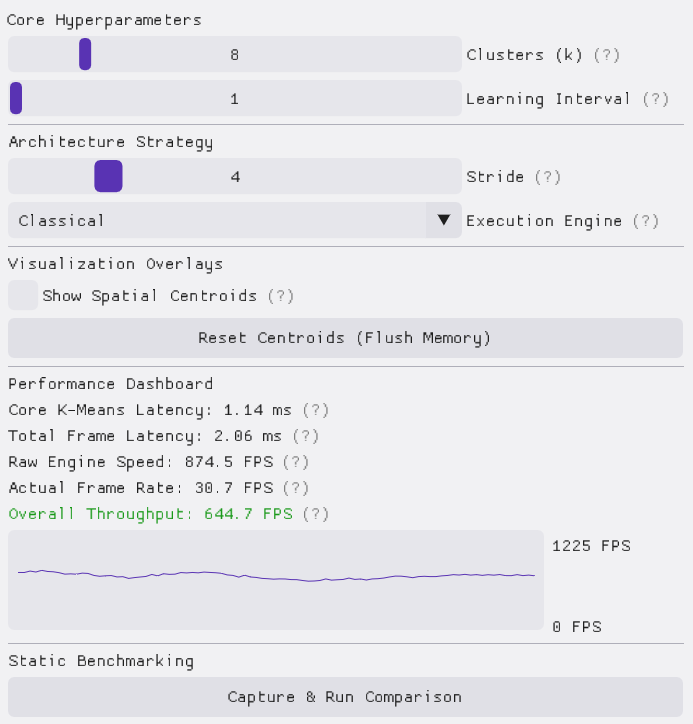
\includegraphics[width=0.7\textwidth]{figures/control_panel.png}
    \caption[Dear ImGui Control Panel]{Dear ImGui control panel and live telemetry dashboard.}
    \label{fig:control_panel}
\end{figure}

\begin{figure}[htbp]
    \centering
    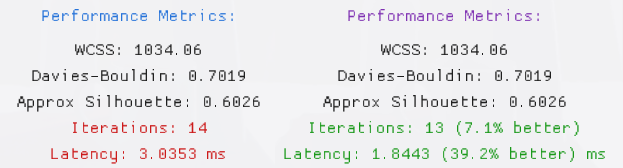
\includegraphics[width=0.8\textwidth]{figures/benchmark_metrics.png}
    \caption[Dear ImGui Benchmarking Telemetry and Speed Metrics]{Dear ImGui benchmarking metrics overlay showing only the comparative execution speed (latency/iterations) and cluster quality measurements for the classical (blue) vs. quantum-inspired (purple) implementations.}
    \label{fig:benchmark_metrics}
\end{figure}

\section{System Interoperability and Communications}
Achieving low latency requires optimizing both the physical transfers across the PCIe bus and the thread synchronization within the application layer.

\subsection{Host-Device Boundary: Heterogeneous Communication}
The main bottleneck in heterogeneous computing is the latency of transferring data across the PCIe bus \cite{CudaGuide}. To minimize this, page-locked (pinned) host memory is used \cite{CudaGuide, cook2012cuda}. Pinned memory enables the GPU to use DMA to copy features directly from host memory without CPU intervention \cite{CudaGuide}. 

Non-blocking asynchronous streams are also used via \texttt{cudaMemcpyAsync} \cite{CudaGuide}. This allows the CPU to continue processing and acquiring the next camera frame while the GPU concurrently runs the active clustering kernel on the current frame \cite{cook2012cuda}.

\subsection{Backend-UI Synchronization}
To keep the GUI running smoothly, the \texttt{ClusteringManager} executes on a dedicated worker thread, preventing heavy GPU computations from blocking the main GLFW render loop \cite{GLFWdocs}. 

Data transfer across this thread boundary is managed using a mutex-protected state machine (\texttt{std::mutex} and \texttt{std::scoped\_lock}) \cite{williams2019c++}. This thread-safe bridge ensures that the UI thread can pull and render the latest visual results, while the worker thread concurrently clusters the next frame, providing flicker-free rendering. The sequence of this multi-threaded execution is visualized in Figure~\ref{fig:thread_sync}. This asynchronous pipeline structure is translated into highly optimized C++/CUDA code in the next chapter, which details the underlying kernel implementations and GPU memory optimization strategies.

\begin{figure}[htbp]
\centering
\resizebox{1\textwidth}{!}{%
\begin{tikzpicture}[
    font=\small,
    lifeline/.style={draw, thick, dashed, gray!60},
    actor/.style={rectangle, draw, rounded corners=3, fill=white, minimum width=2.6cm,
                  minimum height=0.7cm, align=center, font=\small\bfseries, line width=1pt},
    msg/.style={-{Stealth[scale=1.1]}, line width=0.8pt},
    retmsg/.style={-{Stealth[scale=1.1]}, line width=0.8pt, dashed},
    activation/.style={rectangle, draw, fill=gray!15, minimum width=0.22cm},
    notelabel/.style={rectangle, draw=gray!50, fill=yellow!12, rounded corners=2,
                      text width=3.2cm, align=left, font=\scriptsize, inner sep=4pt}
]

% ── Actors ──────────────────────────────────────────────────────────────
\def\GuiX{0}
\def\MutX{5.2}
\def\WrkX{10.4}
\def\TopY{0}
\def\BotY{-11.2}

\node[actor, draw=blue!70,  fill=blue!8 ] (GUI) at (\GuiX, \TopY) {GUI Thread};
\node[actor, draw=orange!80, fill=orange!8] (MTX) at (\MutX, \TopY) {Mutex Bridge};
\node[actor, draw=purple!70, fill=purple!8] (WRK) at (\WrkX, \TopY) {Worker Thread};

% ── Lifelines ────────────────────────────────────────────────────────────
\draw[lifeline] (\GuiX, \TopY-0.35) -- (\GuiX, \BotY);
\draw[lifeline] (\MutX, \TopY-0.35) -- (\MutX, \BotY);
\draw[lifeline] (\WrkX, \TopY-0.35) -- (\WrkX, \BotY);

% ── Messages ─────────────────────────────────────────────────────────────
% 1. GUI acquires config lock
\draw[msg, color=blue!70]
    (\GuiX, -1.2) -- (\MutX, -1.2)
    node[midway, above, font=\scriptsize] {lock(m\_configMutex)};

% 2. GUI writes parameters
\draw[msg, color=blue!70]
    (\GuiX, -2.2) -- (\MutX, -2.2)
    node[midway, above, font=\scriptsize] {write hyperparameters};

% 3. GUI releases lock
\draw[retmsg, color=blue!60]
    (\MutX, -3.0) -- (\GuiX, -3.0)
    node[midway, above, font=\scriptsize] {unlock};

% 4. Worker polls / acquires config lock
\draw[msg, color=purple!70]
    (\WrkX, -4.0) -- (\MutX, -4.0)
    node[midway, above, font=\scriptsize] {lock(m\_configMutex)};

% 5. Worker reads updated params
\draw[retmsg, color=purple!60]
    (\MutX, -4.8) -- (\WrkX, -4.8)
    node[midway, above, font=\scriptsize] {read hyperparameters};

% 6. Worker releases config lock
\draw[retmsg, color=purple!60]
    (\MutX, -5.6) -- (\WrkX, -5.6)
    node[midway, above, font=\scriptsize] {unlock};

% 7. Worker runs CUDA kernels (self-arrow)
\draw[msg, color=purple!80]
    (\WrkX, -6.4) -- ++(0.9,0) -- ++(0,-0.6) -- ++(-0.9,0)
    node[pos=1.0, right=0.95cm, font=\scriptsize, text width=1.8cm] {run K-Means kernels};

% 8. Worker acquires data lock
\draw[msg, color=purple!70]
    (\WrkX, -7.6) -- (\MutX, -7.6)
    node[midway, above, font=\scriptsize] {lock(m\_dataMutex)};

% 9. Worker commits VRAM result
\draw[msg, color=purple!70]
    (\WrkX, -8.4) -- (\MutX, -8.4)
    node[midway, above, font=\scriptsize] {commit staged VRAM data};

% 10. Worker releases data lock
\draw[retmsg, color=purple!60]
    (\MutX, -9.2) -- (\WrkX, -9.2)
    node[midway, above, font=\scriptsize] {unlock};

% 11. GUI pulls texture
\draw[msg, color=blue!70]
    (\GuiX, -10.2) -- (\MutX, -10.2)
    node[midway, above, font=\scriptsize] {lock(m\_dataMutex)};
\draw[retmsg, color=blue!60]
    (\MutX, -10.8) -- (\GuiX, -10.8)
    node[midway, above, font=\scriptsize] {pull texture \& unlock};

\end{tikzpicture}%
}
\caption[Asynchronous Synchronization Sequence between GUI and Worker Threads]{%
    Sequence diagram illustrating asynchronous synchronization between
    the main GUI thread and the clustering worker.}
\label{fig:thread_sync}
\end{figure}